\chapter{The Enigma}

% \begin{chapquote}{Gordon Welchman, \textit{The Hut Six Story Page 52}}
%   The Enigma, though simple in principle and primitive in many ways,
%   presented the cryptanalyst with a dazzling number of possibilities.
% \end{chapquote}
% IMAGES FROM :
% -
% https://www.latimes.com/entertainment/arts/culture/la-et-cm-imitation-game-enigma-machine-david-bohnett-20150122-story.html
% - https://en.m.wikipedia.org/wiki/File:Enigma-plugboard.jpg
% -
% https://en.wikipedia.org/wiki/Enigma_rotor_details#/media/File:Enigma-rotor-pin-contacts.jpg
% -https://en.wikipedia.org/wiki/Enigma_rotor_details#/media/File:Enigma-rotor-flat-contacts.jpg
% -https://en.wikipedia.org/wiki/Enigma_machine#/media/File:Enigma_insides.agr.jpg
% -https://en.wikipedia.org/wiki/File:Enigma_rotor_exploded_view.png
The Enigma machine was used extensively by the Germans to encipher
communications prior to and throughout World War II. German
stratagems like the \emph{blitzkrieg} required quick radio
%% See the Code Book Singh page 196 %%
communication, so to ensure that the allied powers were not able to read
messages, they encoded all radio signals using the Enigma machine.
Breaking the Enigma would allow the allied powers to freely intercept
and decrypt
all naval, air force, and military command -- offering them time to
counter, defend, and retaliate appropriately.
% Thus, while millions
% participated in a war of arms and power, a select group of academics
% at Bletchley Park engaged in a battle of minds to crack a puzzle
% whose solution could save millions of lives.
%https://www.cryptomuseum.com/crypto/enigma/i/index.htm
\section{The Machine}
\begin{figure}[H]
  \begin{center}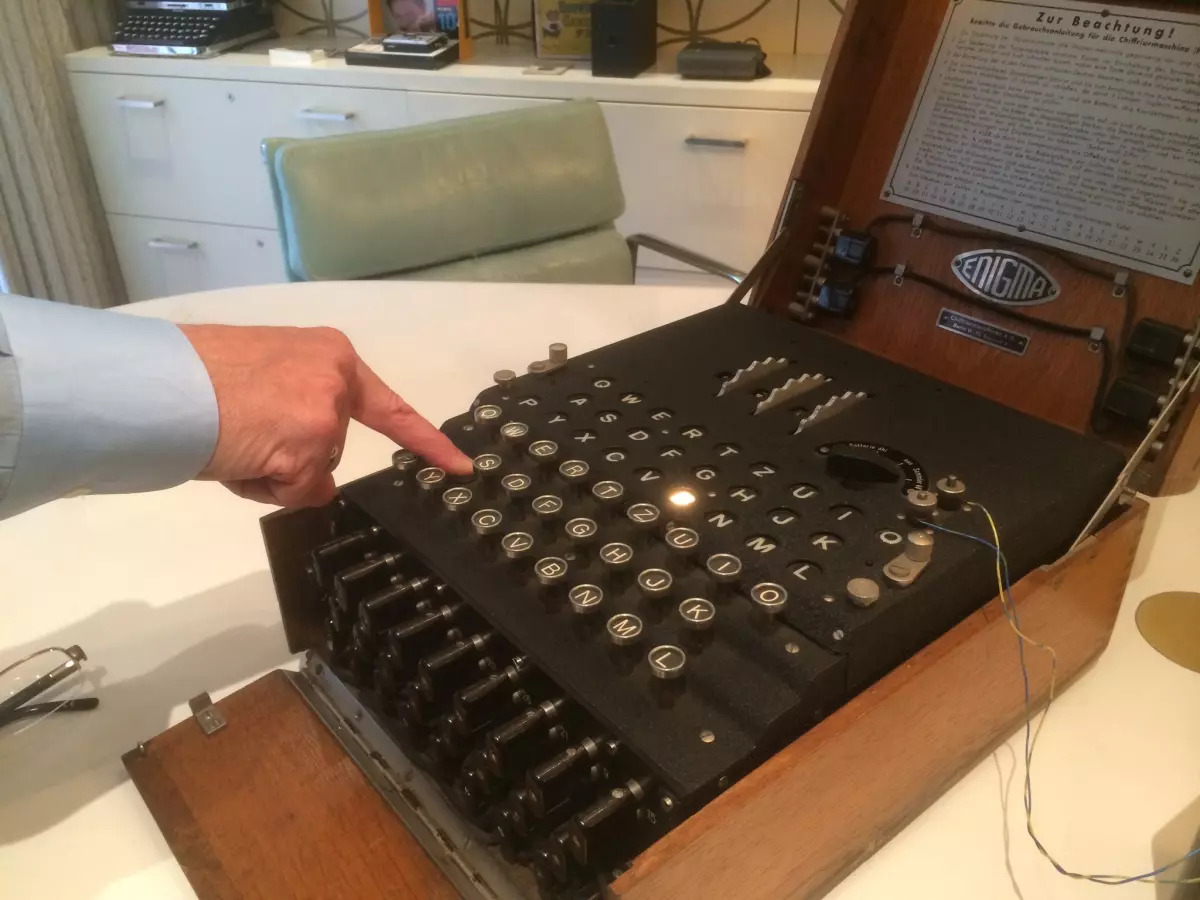
\includegraphics[scale=0.3]{paper/images/enigma.jpg}
  \end{center}
  \label{ref:enigma}
  \caption{Enigma model \texttt{I}}
\end{figure}
Throughout this paper, the model \texttt{I} Enigma is chosen to
represent our canonical machine as this was the most common version
used during World War II with over 20000 being produced~\cite{cryptomuseumEnigmaI}. Further, it
was used by the \emph{Heer} (Army), \emph{Luftwaffe} (Air
Force), and \emph{Kriegsmarine} (Navy), making this a prime target
for attack by cryptanalysts. Many models existed,
each with varying
layouts, key spaces, and use-cases; however, the central ideas that
are discussed in this paper can generally be adapted to work on other models.
\\\\At its most basic function, the Enigma (once set up) is a
keyboard whose letters, when depressed, illuminate bulbs of a
corresponding keyboard layout. The operator presses keys of the
desired plaintext and copies the output of the illuminated bulbs to
obtain the enciphered text. The actual mechanism of this encipherment
requires several mechanical components in a complex arrangement.

\subsection{The Plugboard}

\begin{figure}[htbp]
  \begin{center}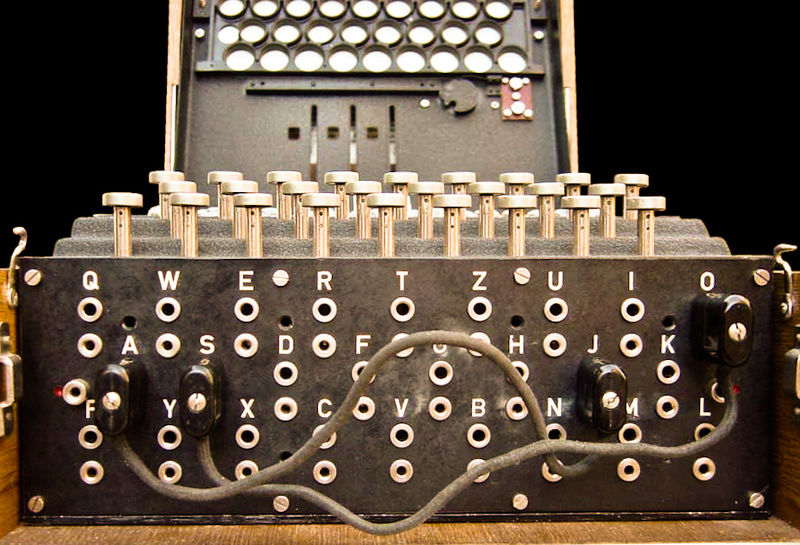
\includegraphics[scale=1.2]{paper/images/plugboard.jpg}
  \end{center}
  \label{ref:plugboard}
  \caption{Enigma plugboard}
\end{figure}
\noindent Upon a key press, the electrical current corresponding to this letter
is sent to a mechanism known as the {\bf{plugboard}}. From an operator's
perspective, the plugboard was a series of ports, one for each
letter, along with 10 cables which could connect these ports. When
two letters are connected via a cable (e.g. A and Z), the plugboard
will send current corresponding to a letter to the opposite letter
(e.g. A goes to Z and vice versa). If no cable is plugged in to a
letter (e.g. D has no cable), then the plugboard simply will return a
current corresponding to this same letter (e.g. D). When a letter is
connected to another
through the plugboard, we will say that the letters are
{\bf{steckered}} to one another. Assuming all 10
cables are used, this means that the plugboard can be represented as a
permutation on 26 letters with $2^{10}1^6$ cycle type\footnote{We
  will denote cycle types in this paper in the format
  $\lambda_1^{m_1}\dots\lambda_k^{m_k}$ where $\lambda_i$ is the length
  of a cycle and $m_i$ is the multiplicity of this cycle length. We
  will often write the full notation $1^{m_1}\dots n^{m_n}$ in which
$m_i$ may be $0$.}. One such
permutation could be
\begin{center}
  (\texttt{HR})(\texttt{AT})(\texttt{IW})(\texttt{SK})(\texttt{UY})(\texttt{DF})(\texttt{GV})(\texttt{LJ})(\texttt{BQ})(\texttt{MX})(\texttt{C})(\texttt{E})(\texttt{N})(\texttt{O})(\texttt{P})(\texttt{Z}).
\end{center}
In general, we will denote the permutation corresponding to a plugboard as $S$.

\subsection{The Rotors}

\begin{figure}[H]
  \centering
  \begin{minipage}{0.48\textwidth}
    \centering
    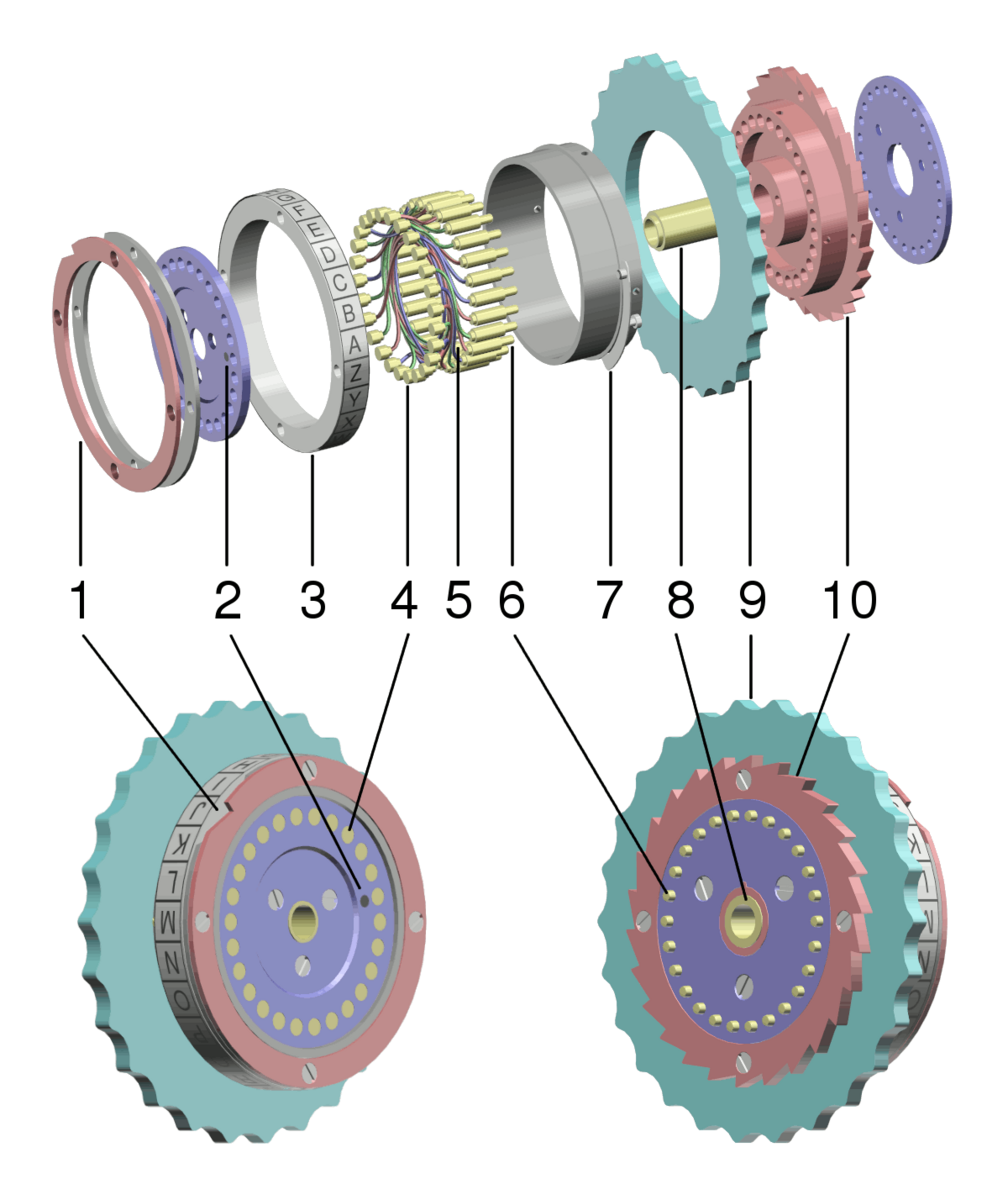
\includegraphics[width=\linewidth]{paper/images/disassembled.png}
    \subcaption{Disassembled rotor}
  \end{minipage}%
  \hfill
  \begin{minipage}{0.48\textwidth}
    \centering
    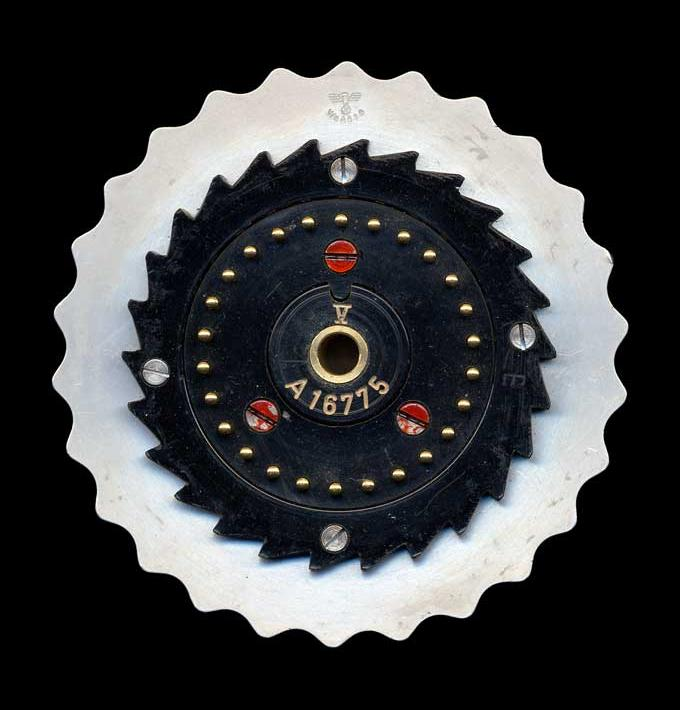
\includegraphics[width=0.8\linewidth]{paper/images/entry.jpg}
    \subcaption{Enigma rotor \texttt{V} entry side}
    \vspace{4mm} % adjust spacing as needed
    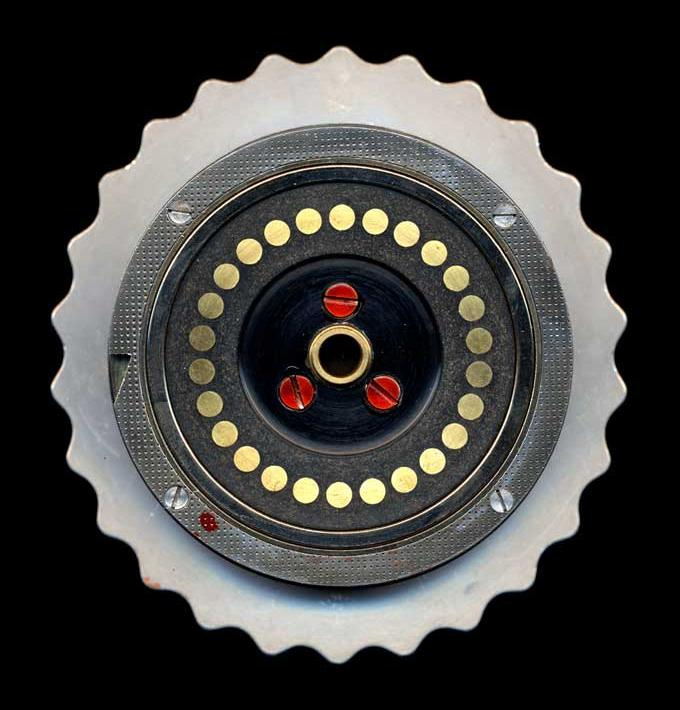
\includegraphics[width=0.8\linewidth]{paper/images/exit.jpg}
    \subcaption{Enigma rotor \texttt{V} exit side}
  \end{minipage}
  \caption{Enigma rotor}
  \label{fig:rotors}
\end{figure}
% \begin{figure}[htpb]
%   \centering
%   \begin{subfigure}{0.3\textwidth}
%     \includegraphics[width=\linewidth]{images/rotor_v_front.jpg}
%     \caption{Entry-side}
%     \label{fig:rotor_v_front}
%   \end{subfigure}
%   \hspace{0.02\textwidth}
%   \begin{subfigure}{0.3\textwidth}
%     \includegraphics[width=\linewidth]{images/rotor_v_back.jpg}
%     \caption{Exit-side}
%     \label{fig:rotor_v_back}
%   \end{subfigure}
%   \caption{Rotor \texttt{V}}
%   \label{fig:rotor_v}
% \end{figure}

The Enigma model \texttt{I} used three rotors, selected from a larger
set of rotors, the number of which changed depending on the military
branch we examine. At a minimum, all three branches of the military eventually
had access to five rotors labeled by their roman numeral equivalents
(i.e. $\texttt{I},\dots,\texttt{V}$).
Each rotor encoded a unique permutation from 26 input contacts to 26
output contacts by simply connecting each input/output pair
in the permutation with a wire as in figure~\ref{fig:rotors}
(a)-(4,5,6). The contacts represent the letters
in alphabetical order moving in a clockwise manner relative to the
entry side of the rotor. The input contacts of the rotor were often marked
with a white dot indicating which contact corresponded to \texttt{A},
but in general the \texttt{A} contact found by looking at the contact immediately above
the numeral indicator as in figure~\ref{fig:rotors} (b).
\\\\On their own, these rotors would prove to be very poor
cryptographic devices, as they are just substitution ciphers, which are
vulnerable to frequency analysis and, if found by the enemy, would
serve no purpose whatsoever. Therefore, these rotors were designed to
rotate, which served to change the substitution at each stage of encryption.
\\\\Because these rotors rotate, it is best to differentiate between
contact letters and contact positions. When we give the permutation
corresponding to a rotor as in figure \ref{fig:rotor_v_wiring} we are
referring to the \texttt{A} contact as the specific contact denoted
by the marker dot and the \texttt{B} contact as its next contact
turning clockwise. When referred to in this context, we will use the
word ``contact.'' On the other hand, when we say that an electrical
current corresponding to \texttt{A} enters a rotor, we mean
that the current enters the contact at the topmost \emph{position} of
the rotor, even if the rotor has rotated now so that that contact
is not the contact with the marker dot. When referred to in this
context we will use the word ``position'' so as to disambiguate from
the prior context. That is to say, a contact and a position need not
be the same. For example, contact \texttt{A} can be in position
\texttt{B}. This occurs when the pin with the marker dot adjacent to
it is one pin away from being at the top of the rotor.

\subsubsection{Turnover}
Each rotor had on its entry-side, a notch next to each contact as in
figure~\ref{fig:rotors} (b). A pawl
attempted to engage
the notch and move the rotor forward by one contact each key press.
On the exit-side, each
rotor was equipped with a smooth ring with only a single notch
breaking it as in figure~\ref{fig:rotors} (c). This is known as the
{\bf{turnover notch}}. Assuming the
rotor functions in isolation the pawl will engage the entry notches
during each key press thus moving the rotor forward by one until,
after 26 presses, the rotor returns to its original position.
However, if we have two rotors, say rotor M and N, such that rotor M
has its entry contacts placed adjacent to the exit contacts of rotor
N; then, the smooth ring of the rotor N will occlude the notches of
rotor M thus preventing the pawl from engaging. That is, except at
the location where the turnover notch is located. The pawl will then
only be able to rotate rotor M if it aligns with the turnover notch of rotor N.
\\\\Now consider three rotors, rotors L, M, and N, arranged left to
right from an operator's perspective. Then electrical current first
enters rotor N, followed by rotor M, and finally rotor L. Rotor N
will have no rotor's smooth ring occluding its notches so the pawl is
free to engage rotor N at every key press. Thus rotor N will always
turn at each press of the key. Rotor M, however, will only turn at
the position at which rotor N's turnover notch aligns with the pawl
(save for a case we will shortly discuss),
meaning that for each full rotation of rotor N, rotor M will move
by one contact. Finally, rotor L will only move when rotor M's
turnover notch is aligned with the pawl, meaning that rotor N must
make 26 full rotations before rotor L will move by one contact.

%% https://www.cryptomuseum.com/crypto/enigma/m3/index.htm %%
\begin{center}
  \begin{figure}[h]
    \[
      \left(
        \begin{array}{llllllllllllllllllllllllll}
          \texttt{A} & \texttt{B} & \texttt{C} & \texttt{D} &
          \texttt{E} & \texttt{F} & \texttt{G} & \texttt{H} &
          \texttt{I} & \texttt{J} & \texttt{K} & \texttt{L} &
          \texttt{M} & \texttt{N} & \texttt{O} & \texttt{P} &
          \texttt{Q} & \texttt{R} & \texttt{S} & \texttt{T} &
          \texttt{U} & \texttt{V} & \texttt{W} & \texttt{X} &
          \texttt{Y} & \texttt{Z}                             \\
          \texttt{V} & \texttt{Z} & \texttt{B} & \texttt{R} &
          \texttt{G} & \texttt{I} & \texttt{T} & \texttt{Y} &
          \texttt{U} & \texttt{P} & \texttt{S} & \texttt{D} &
          \texttt{N} & \texttt{H} & \texttt{L} & \texttt{X} &
          \texttt{A} & \texttt{W} & \texttt{M} & \texttt{J} &
          \texttt{Q} & \texttt{O} & \texttt{F} & \texttt{E} &
          \texttt{C} & \texttt{K}
        \end{array}
      \right)
    \]
    \caption{Rotor \texttt{V} permutation}
    \label{fig:rotor_v_wiring}
  \end{figure}
\end{center}

\subsubsection{Double Stepping}\label{double_step}
Arguably the most confusing aspect of the mechanics of the Enigma
machine is that of the {\bf{double step}}. We just said that the each
of the left two rotors ($M$ and $L$) can \emph{only} be moved when
the turnover notch of its right-hand adjacent rotor ($N$ and $M$
respectively) is aligned with the pawl. For $L$ this is true.
However, for rotor $M$, we must consider that even if rotor $N$'s
turnover notch is \emph{not} aligned with the pawl, rotor $M$'s own
turnover notch \emph{may} be aligned with the pawl. In this case, the
pawl will engage and move $L$; however, the turnover notch is still
connected to rotor $M$, so when the pawl engages $M$'s turnover notch
it will not only move $L$, but it will also move $M$ (just from the
opposite side that we might expect).
\\\\We will illustrate this effect by example. Suppose our rotors
$N$, $M$, and $L$ had only three positions ($1$, $2$, and $3$). They
will each have a turnover notch aligned with a pawl when at position
$1$. We will walk through a full cycle of turnover of the leftmost
rotor $L$ step-by-step. We have
\begin{itemize}
  \item (Step $0$) $L = 2$, $M = 2$, $N = 3$ -- This represents our
    initial position
  \item (Step $1$) $L = 2$, $M = 2$, $N = 1$ -- Pawl engages $N$ and
    steps it forward
  \item (Step $2$) $L = 2$, $M = 3$, $N = 2$ -- Pawl engages $N$ and
    $N$'s turnover notch engages $M$.
  \item (Step $3$) $L = 2$, $M = 3$, $N = 3$ -- Pawl engages $N$ and
    steps it forward
  \item (Step $4$) $L = 2$, $M = 3$, $N = 1$ -- Pawl engages $N$ and
    steps it forward
  \item (Step $5$) $L = 2$, $M = 1$, $N = 2$ -- Pawl engages $N$ and
    $N$'s turnover notch engages $M$.
  \item (Step $6$) $L = 3$, $M = 2$, $N = 3$ -- Pawl engages $N$.
    $M$'s turnover notch engages $L$ but this also has the effect of
    rotating $M$ as well, even though $N$'s turnover notch is
    \emph{not} aligned. Observe that $M$ has now moved twice in two
    steps, hence the name ``double step''.
\end{itemize}
From this example, we note that on an Enigma with 26 letters, the
leftmost rotor $L$
moves every $26\cdot25$ steps. We might expect this to occur every
$26\cdot26$ steps, but
because of double stepping the period is shortened.
\subsubsection{Rotation}

Consider the effect of a rotor turn on rotor \texttt{V}, whose
internal wiring is described in figure \ref{fig:rotor_v_wiring}.
In a default position in which contact \texttt{A} is at position
\texttt{A}. After pressing a key, the rotor
will turn resulting in contact \texttt{B} now being in position
\texttt{A}. This means that an input current
entering at position \texttt{A} will go into contact \texttt{B}, be
routed through the permutation and exit at contact
\texttt{Z} which now is at position \texttt{Y} due to the rotation.
This is to say that rotating the rotor has the effect
of shifting an input letter forward by 1 (mod 26) and the output
letter back by 1 (mod 26).
\\\\To encode the effect of rotation as a permutation consider
\begin{definition}
  The \emph{Caesar permutation} (denoted $P$) is the permutation
  taking a letter to the next letter in alphabetical order (mod 26).
  Its two-line permutation notation is
  \[
    \left(
      \begin{array}{llllllllllllllllllllllllll}
        \texttt{A} & \texttt{B} & \texttt{C} & \texttt{D} &
        \texttt{E} & \texttt{F} & \texttt{G} & \texttt{H} &
        \texttt{I} & \texttt{J} & \texttt{K} & \texttt{L} &
        \texttt{M} & \texttt{N} & \texttt{O} & \texttt{P} &
        \texttt{Q} & \texttt{R} & \texttt{S} & \texttt{T} &
        \texttt{U} & \texttt{V} & \texttt{W} & \texttt{X} &
        \texttt{Y} & \texttt{Z}                             \\
        \texttt{B} & \texttt{C} & \texttt{D} &
        \texttt{E} & \texttt{F} & \texttt{G} & \texttt{H} &
        \texttt{I} & \texttt{J} & \texttt{K} & \texttt{L} &
        \texttt{M} & \texttt{N} & \texttt{O} & \texttt{P} &
        \texttt{Q} & \texttt{R} & \texttt{S} & \texttt{T} &
        \texttt{U} & \texttt{V} & \texttt{W} & \texttt{X} &
        \texttt{Y} & \texttt{Z} & \texttt{A}
      \end{array}
    \right).
  \]
\end{definition}
\noindent If we denote the permutation corresponding to rotor \texttt{V} in
default position as $\eta$. Then after $r$ rotations, to get
our new permutation we must first shift each input letter forward by
$r$ and each output letter backwards by $r$. This can be encoded via
the Caesar permutation as follows
\[
  {P^{-r}}\eta{P^{r}}.
\]x
\noindent It should be noted that current will only flow through the
machine \emph{after} the rotation has taken place. Thus encrypting a
letter with the window indicating \texttt{AAA} is really going to
send current through the rotors with the window indication
\texttt{AAB} since the rightmost rotor will turn before the encryption happens.
\subsubsection{Outer Ring}

The rotors were additionally equipped with an outer ring with
letters \texttt{A} to \texttt{Z} moving clockwise relative to the
entry-side of the rotor as in figure~\ref{fig:rotors} (a)-(3).
Alternately some rings had numerical values
ranging from \texttt{01} to \texttt{26}. The outer ring was not fixed
to the underlying rotor and could be moved. Most importantly, this
outer ring is what contained the turnover notch -- that is, the
component in figure~\ref{fig:rotors} (a)-(3) was connected to the
component (a)-(1). Thus, by moving the outer ring, we change where
turnover occurs relative to the internal wiring of the rotor.
\\\\To consider the effect of this ring,
consider if an operator were instructed to place the ring such that
the outer ring's \texttt{02} label was placed over contact \texttt{A}. Once
the rotor is closed inside the machine
the operator can now only see the letters indicated by the outer ring
appearing in a small window. If he moves the ring's label \texttt{01}
to be in the window, then contact \texttt{Z} is now in position
\texttt{A}. This means that an input current
entering at position \texttt{A} will go into contact \texttt{Z}, be
routed through the permutation and exit
at contact \texttt{K} which now is at position \texttt{L} due to the
ring setting. This is to say that moving the ring
setting has the effect of shifting an input letter back by 1 (mod 26)
and the output letter forward by 1 (mod 26).
As in the prior discussion on rotor rotation, if we denote the
permutation corresponding to rotor \texttt{V} in default position as
$\eta$. Then shifting the ring by $r$ letters, we get a new
permutation by first shifting each input letter backwards by $r$ and
each output letter forwards by $r$. This can be encoded via the
Caesar permutation as follows
\[
  {P^{r}}\eta{P^{-r}}.
\]
In this sense, we can think of rotor rotations and ring adjustments
as having inverse effects. In fact, if we ignore turnover, setting
the ring forward by $r$ letters and then rotating the rotor forward by $r$
letters is equivalent to having left the ring setting and rotor in
its default position. That is to say, for cases where turnover does
not occur, the ring setting (\emph{Ringstellung}) and which letter
we decide to show in our window (\emph{Grundstellung}) really
represent one singular component of our key space since we can always
consider our ring setting as being at \texttt{A} by just shifting
which letter we display in our window.
However, consider that changing the ring
setting also changes where the turnover occurs relative to the
internal wiring of a rotor. This means that for rotors $M$ and $L$
which are affected by turnover, the ring setting does add to
the key space since it has effects which are independent of the
window setting.

%% NOTE HAPPENES AFTER PAWL %%

% In default position the effect of this ring is just that it conveys
% which contact corresponds to which letter and, when the rotors are
% locked inside the Enigma machine, displays to the operator which
% letter is at the top of the rotor through a small window for each
% rotor. However, the ring itself was disconnected from the rotor and
% could be rotated freely. Further, the turnover notch moved along with
% the ring and thus changing the ring setting would also change the
% relative turnover point for each rotor.
% This has two effects.
% \begin{itemize}
%   \item If the operator is instructed to use rotor \texttt{V} and to
%         have \texttt{A} showing through the window on their machine then
%         if the ring setting is such that \texttt{A} on the ring
%         corresponds to contact letter \texttt{A} (the contact next to the
%         marker dot), then a current entering at the position
%         correpsonding to \texttt{A} will exit at the position
%         corresponding to \texttt{E}; however, if the ring setting is such
%         that \texttt{A} on the ring corresponds to contact letter
%         \texttt{B}, then a current entering at the position corresponding
%         to \texttt{A} will exit at the position corresponding to
%         \texttt{K} . In this sense the, ring setting has an inverse
%         relationship to how much the rotor has turned. If the rotor has
%         turned by one contact, but the ring setting has been turned by
%         one letter from the default position, then, as a permutation, it
%         is as if the rotor has a default ring setting and has not moved.
% \end{itemize}

\subsection{The Reflector}
\begin{figure}[H]
  \begin{center}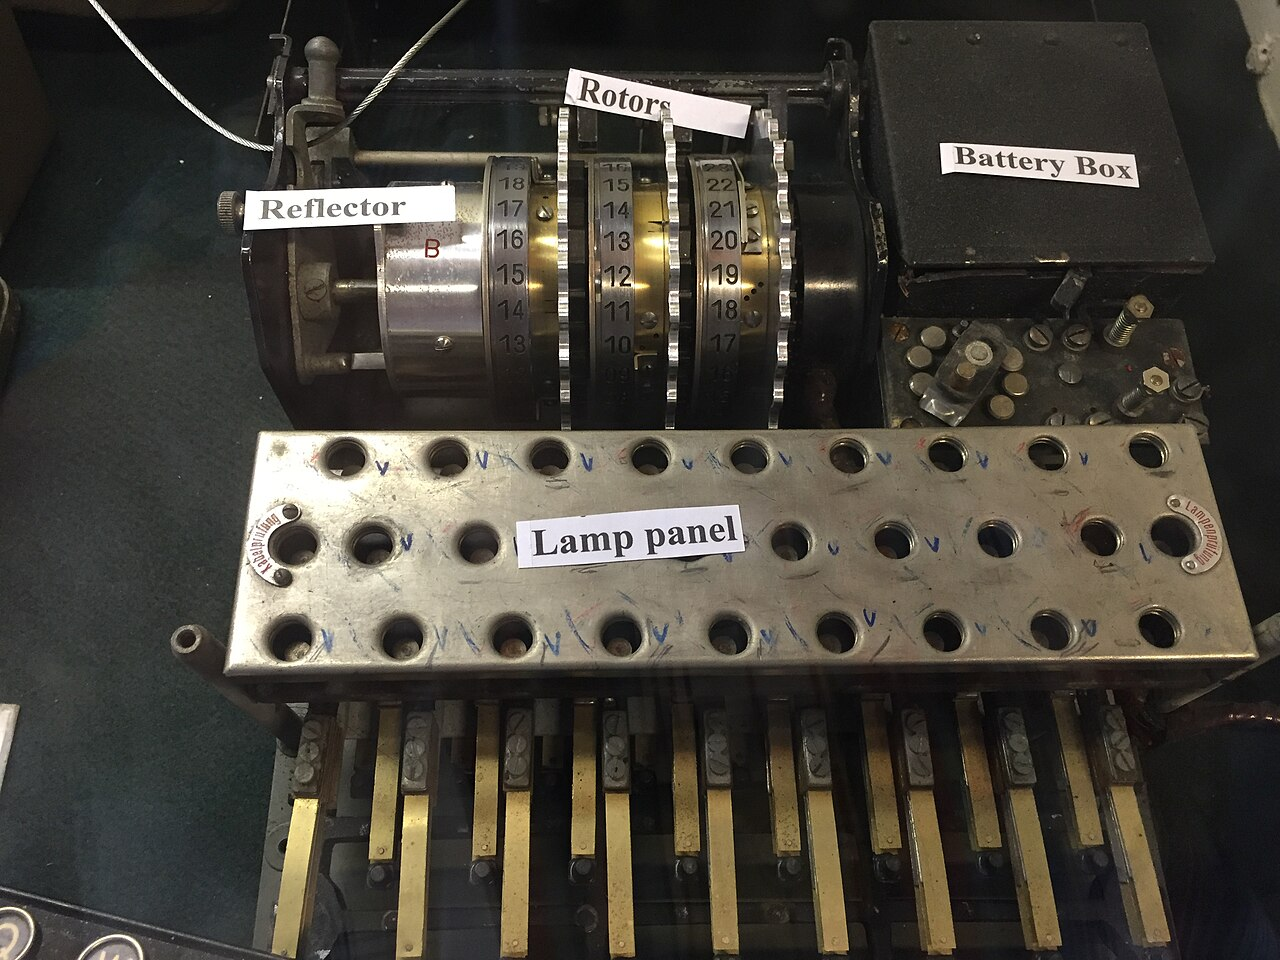
\includegraphics[scale=0.3]{paper/images/internals.jpg}
  \end{center}
  \label{ref:internals}
  \caption{Enigma internals illustrating reflector placement}
\end{figure}
\noindent After the current travels through all three rotors, it ends up at the
reflector which we will denote $R$. The reflector is specially
designed so that its permutation consists only of disjoint
transpositions, that is it has a $2^{13}$ cycle type. This means that
reflector simply swaps letters in a set of $13$ pairs.
\\\\Rather than having an entry and an exit side each with their own
contacts, the reflector has one side of contacts. Current enters at a
particular contact and is routed through the permutation back out
this same side at a different contact. The reason for this is that
the reflector's job is to send current through the exact inverse of
the process we have described up to this point. That is, after
exiting the reflector, current travels back through the rotors (now
entering at the exit contacts of the leftmost rotor), travels back
through the plugboard, and now ends up at a lamp light indicating the
enciphered letter.

\section{Key Size}

\subsubsection{\emph{Plugboard Setting (}Steckerverbindungen\emph{)}}
10 plugboard wires are selected in total. The first wire must connect
2 out of 26 letters giving us ${26\choose2}$ locations this wire can
be placed. We now select a wire for the next two letters giving us
${24\choose2}$ remaining locations. We continue in this fashion until
having placed 9 wires leaving us ${8\choose2}$ remaining choices. In
total, we have found
\begin{align*}
  & {26\choose2}{24\choose2}\dots{8\choose2}                                  \\
  & =\frac{26!}{2!\cdot 24!}\frac{24!}{2!\cdot 22!}\dots\frac{8!}{2!\cdot 6!} \\
  & =\frac{26!}{2^{10}\cdot6!}
\end{align*}
possible wire arrangements. Of course, the order in which we select
the 10 wires does not matter so we have over-counted and must
therefore divide this value by $10!$ wire orderings. Therefore, we have
\[
  \frac{26!}{2^{10}\cdot 10! \cdot 6!}
\]
plugboard settings.

\subsubsection{\emph{Rotor Selection (}Walzenlage\emph{)}}
From the 5 rotors in circulation, 3 rotors in some order were needed
to operate the Enigma machine. There are thus ${5}\choose{3}$ total
selections of 3 rotors each of which can be ordered in $3!$ ways,
giving us ${5\choose3}\cdot{3!}$ possibilities.

\subsubsection{\emph{Ring Setting (}Ringstellung\emph{)}}
Recall that the only rotors for which the ring setting actually adds
to the keyspace is the 2 rightmost rotors since this setting changes
where turnover occurs and only the 2 leftmost rotors are affected by
turnover. Since each ring can be setting corresponds a letter from
the 26 letter alphabet, this gives us $26^2$ possibilities.

\subsubsection{\emph{Window Setting (}Grundstellung\emph{)}}
A window setting specified 3 letters from the 26 letter alphabet
giving us $26^3$ possibilities.

\subsubsection{\emph{Reflector Selection}}
While there are multiple reflectors each of which saw varying levels
of usage during World War II, most machines generally stuck to a
fixed reflector known as \texttt{UKW-B}. Therefore, this does not
factor into our key space but is worth noting if other reflectors are
being considered.

\subsubsection{Total Key Size}
Putting together all these components of an Enigma's key settings we
derive the following expression for the total number of keys
\[
  \frac{26!}{2^{10}\cdot 10! \cdot 6!}\cdot{5\choose 3}\cdot3!\cdot
  26^2\cdot 26^3 \approx 1.07 \cdot 10^{23} \approx 2^{77}
\]
resulting in a roughly $77$-bit key space.
\\\\With such a large key space, it seemed to the Germans that Enigma
was unbreakable. This was an era before computers could churn through
massive key spaces in a matter of hours. Any attempt to break Enigma
was going to require an attack more intelligent than brute-forcing.
\\\\In Chapter 2, we will see how Polish cryptanalyst made use of a
flaw in the Enigma protocol, along with some clever mathematics, to
construct one of the earliest attempts at breaking the cipher. To
provide the requisite background, we will examine the protocol by
which German Enigma operators sent messages, as well as provide a
mathematical formalism for the machine.

\section{The Enigma Protocol}\label{protocol}
%% https://bletchleypark.org.uk/our-story/enigmas-of-bletchley-park/%%
%% https://www.cryptomuseum.com/crypto/enigma/i/index.htm%%
%% https://www.cryptomuseum.com/crypto/enigma/files/schluessel_m.pdf%^

%% FOR THE DATE GET
% chrome-extension://efaidnbmnnnibpcajpcglclefindmkaj/https://www.math.ias.edu/files/wam/rejewski.pdf
% $$
Suppose Alice and Bob are two radio operators (prior to September 15,
1938) who want to communicate securely. Each are supplied an Enigma
machine along with a key sheet indicating the keys for a given day.
The key sheet contains the following information:
\begin{itemize}
  \item the choice and order of rotors, known as the
    \emph{Walzenlage} -- at this point only three
    rotors \texttt{I}, \texttt{II}, and \texttt{III} were in
    production,
  \item the ring setting, known as the \emph{Ringstellung},
    %% See rejwinski for this %%
  \item the plugboard settings, known as the
    \emph{Steckerverbindungen} -- at this point only 3 jacks were used

  \item the window setting, known as the \emph{Grundstellung}.
\end{itemize}
A key sheet at this time may have looked along these lines.

\begin{figure}[H]
  \begin{center}
    \resizebox{0.98\textwidth}{!}{
      \begin{tabular}{|c|c|c|c|c|}
        \hline
        \textbf{\emph{\texttt{Datum}}}               &
        \textbf{\emph{\texttt{Walzenlage}}}          &
        \textbf{\emph{\texttt{Ringstellung}}}        &
        \textbf{\emph{\texttt{Steckerverbindungen}}} &
        \textbf{\emph{\texttt{Grundstellung}}}
        \\
        \hline
        \texttt{31.}                                 & \texttt{I II
        III}                                         & \texttt{10 14
        02}                                          & \texttt{BF SD
        AY}                                          & \texttt{VAR}
        \\
        \texttt{30.}                                 & \texttt{I II
        III}                                         & \texttt{04 25
        01}                                          & \texttt{UE PL
        AY}                                          & \texttt{PAQ}
        \\
        \texttt{29.}                                 & \texttt{I II
        III}                                         & \texttt{13 11
        06}                                          & \texttt{WJ VD
        PO}                                          & \texttt{ZJB}
        \\
        $\vdots$                                     & $\vdots$
        & $\vdots$      & $\vdots$ & $\vdots$ \\
        \hline
    \end{tabular}}
  \end{center}
  \caption{Mock Enigma key sheet pre-1938}
  \label{fig:keysheet_early}
\end{figure}

\noindent Alice wants to encrypt the message \texttt{HELLO WORLD} on
the 31st of the month using the key sheet in figure
\ref{fig:keysheet_early}. She opens the machine and places the rotors in
the machine from left to right as \texttt{I}, \texttt{II},
\texttt{III}\footnote{Prior to January 1, 1936, the sequence of
rotors was only changed once a quarter}. She then aligns the
\texttt{10} indicator on the
leftmost drum to be inline with the \texttt{A} contact, and similarly
for the remaining ring settings. Alice now closes the machine and
rotates the rotors so that they display \texttt{VAR} (or in numerals
\texttt{22} \texttt{01} \texttt{18}) in the window of
each rotor. Finally, Alice connects \texttt{B} and \texttt{F} in the
plugboard and similarly for the remaining plugboard settings. Alice
now chooses a random message key, this is a three letter trigram
called the \emph{Spruchschlüssel}. Alice chooses her message key as
\texttt{LSG} and is now ready to encrypt her message.
\\\\First, Alice will encrypt her message key \texttt{LSG} twice,
producing the hexagram
\begin{center}
  \texttt{KUW ACQ}
\end{center}
\noindent Alice now sets her window setting to her message key
\texttt{LSG} and begins enciphering her message \texttt{HELLO WORLD} to produce
\begin{center}
  \texttt{WQMYV HWGAB}
\end{center}
Alice now sends the following message to Bob
\begin{center}
  \texttt{KUW ACQ WQMYV HWGAB}
\end{center}
\noindent Bob recieves this message. He gets his key sheet and sets
up his machine as the key sheet describes for that day. He now types
in the first six letters of the message to get back Alice's message
key, which will look like
\begin{center}
  \texttt{LSG LSG}
\end{center}
We can now see why we doubly encoded the message key. If Bob did not
see the same trigram repeated twice he would know that either he or
Alice set up their machine incorrectly, or that Alice incorrectly typed in
her message key. Bob could then tell Alice to correct the message.
Now equipped with Alice's message key, Bob sets his machine window to
\texttt{LSG} and begins typing in the remainder of the message to
recover the plaintext
\begin{center}
  \texttt{HELLO WORLD}
\end{center}
\noindent It should be noted, the procedure described here is a
facsimile of the actual procedure meant to only convey the components
that are cryptographically significant. In practice, additional
information was sent alongside the message such as time of
transmission and radio station of origin. Further the message itself
was to be encoded with particular rules, for example, spaces would be
denoted with \texttt{X}. As we discuss changes to Enigma protocol
throughout this paper we will leave such details out.
%% https://www.ilord.com/enigma-manuals %%
%% REAL DECRYPT FOR EXAMPLE OH WAIT THESE MIGHT JUST BE TUNNY
% DECRYPTS
% https://web.archive.org/web/20160406042455/http://www.ilord.com/bp-decrypts.html
% %%
% Further, each have a copy of the ``\emph{Gebrauchsanleitung für die
% Chiffriermaschine Enigma}'' -- a book entailing all the protocols
% necessary for Alice
% and Bob to communicate securely. The manual explains
% \\\\\texttt{III. Setting the Key. }
% \\\texttt{10. The codebook issued with the machine determines the
% following 4 settings of the device:}
% \\\texttt{1. Order of the encryption rotors (III/IV, 12) (\emph{Walzenlage}),}
% \\\texttt{2. Setting of the number or letter rings( III/IV, 13) on
% the 3 encryption rotors (\emph{Ringstellung}),}
% \\\texttt{3. Setting of the numbers or letters visible in the
% windows (I/II, 16) (\emph{Grundstellung}),}
% \\\texttt{4. Establishment of the connections using the patchcords
% (II, 30) on the plug board (II, 15) (\emph{Steckerverbindungen}).}

%% FOR PROTOCOL NOTE FROM CODE BOOK TAHT CERTAIN SCRAMBLER POSITIONS
% WERE DISALLOWED YAY OR CERTAIN PLUGBOARD SETTINGS %%

\section{Enigma as a Permutation}

Recall that from the keyboard, current will enter the plugboard
($S$), followed by the rigtmost rotor ($N$), middle
rotor ($M$), leftmost rotor ($L$), and the reflector ($R$), only to
return through each of these components. Then at default position the
Enigma machine can be represented as a permutation
\[
  \pi_0 \coloneq S^{-1}N^{-1}M^{-1}L^{-1}RLMNS
\]

\noindent Additionally recall that if we ignore turnover the ring setting and
window setting effectively represent one singular setting.
Then, by proper adjustment of permutations ($L$, $M$, and $N$) we can
consider any Enigma setting as beginning in such a state as described
by $\pi_0$. Further, each subsequent key-press will bring us to a new
state with a new permutation given by
\[
  \pi_i \coloneq S^{-1}P^{i}N^{-1}P^{-i}M^{-1}L^{-1}RLMP^{-i}NP^{i}S
\]
where $i$ describes the number of times we have depressed the
keyboard. Of course, turnover does exist and does matter; however, if
we are examining only the first few letters (say $l$) of a message
being encrypted, we have a $\frac{25}{26}$ chance of no turnover
occurring at each step and so we have a $(\frac{25}{26})^l$ chance of
no turnover occurring during our initial stages on encryption. For
small $l$ this is a reasonably high probability. We will see that the
first Enigma codebreakers made use of this
fact to simplify their model of the machine to the above permutation $\pi_i$.

\subsection{Cycle Type}
Consider the structure of the permutation $\pi_i$. We have
\begin{align*}
  \pi_i & = S^{-1}P^{i}N^{-1}P^{-i}M^{-1}L^{-1}RLMP^{-i}NP^{i}S \\
  & = (LMP^{-i}NP^{i}S)^{-1}R(LMP^{-i}NP^{i}S).
\end{align*}
That is, $\pi_i$ is simply the reflector permutation $R$
pre-composed and post-composed with a permutation and its inverse
respectively. This leads us to the following definition,

\begin{definition}
  Let $G$ be a group. We say two elements $a,b\in{G}$ are
  {\bf{conjugate}} if $\exists\text{ }g\in{G}$ s.t. $a=gbg^{-1}$.
\end{definition}
\text{}\\In this way, we can shorten our above observation to say that
$\forall\text{ }i\in\mathbb{N}$ we have that $\pi_i$ and $R$ are
conjugate permutations. This point is true regardless of turnover
since the permutations being pre-composed and post-composed with $R$
are always inverse permutations. Now consider the following lemma,\\
\begin{lemma}
  Suppose $\rho=(a_0\dots a_{k-1})\in S_n$ is a $k$-cycle. Then
  $\forall\text{ }\tau\in S_n$ we have
  $\tau\rho\tau^{-1}$ is a $k$-cycle.
  \label{conjugate_cycle}
\end{lemma}
\begin{proof}
  Since $\tau\in S_n$ is a bijection, to show how $\tau\rho\tau^{-1}$
  acts on $\{1,\dots, n\}$ it suffices to show how it acts on
  $\{\tau(1), \dots, \tau(n)\}$.
  We consider how $\tau\rho\tau^{-1}$ acts on elements of the form
  $\tau(a_i)$ for a fixed $i\in\{0,\dots,k-1\}$.
  \begin{align*}
    \tau(a_0\dots a_{k-1})\tau^{-1}(\tau(a_i)) & = \tau(a_0\dots
    a_{k-1})(a_i)
    \\
    & = \tau(a_{(i+1)\text{ mod }k}) \\
  \end{align*}
  Then we know $\tau\rho\tau^{-1}$ contains the cycle
  $(\tau(a_0)\dots \tau(a_{k-1}))$.
  Further, if $\tau\rho\tau^{-1}$ acts on the remaining elements
  $\tau(x)$ where $x\in\mathbb{N}_N - \{a_0,\dots,a_{k-1}\}$.
  Then we have
  \begin{align*}
    \tau(a_0\dots a_{k-1})\tau^{-1}(\tau(x)) & = \tau(a_0\dots a_{k-1})(x) \\
    & = \tau(x)                   \\
  \end{align*}
  Meaning $\tau\rho\tau^{-1}$ acts as the identity on $\tau(x)$. From
  this we can deduce that
  $\tau\rho\tau^{-1}$'s cycle decomposition consists of a single
  cycle of length $k$.
\end{proof}

\noindent This lemma leads us to the following theorem that will be of deep
relevance for the remainder of the paper.

\begin{theorem}
  \label{conjugate_cycle_type}
  $\forall\text{ }\alpha, \beta \in S_n$ we have
  \begin{center}
    $\alpha$ and $\beta$ are conjugates $\iff$ $\alpha$ and $\beta$
    have the same cycle type~\cite{ProofWikiConjugateCycleType}.
  \end{center}
\end{theorem}
\begin{proof}
\text{}\\$\Rightarrow$) Suppose $\exists\text{ }\tau\in S_n$ s.t.
$\alpha = \tau\beta\tau^{-1}$. $\beta$ has some cycle type
$1^{m_1}\dots n^{m_n}$. We can decompose
$\beta$ into disjoint cycles $\beta_{i,j}$ for $i\in\mathbb{N}_n$ and
$j\in\mathbb{N}_{m_i}$. That is, there are $m_i$ cycles $\beta_{i,j}$
of length $i$. We then have,
\begin{align*}
  \alpha & = \tau\beta\tau^{-1}
  \\
  & =
  \tau\bigl(\beta_{1,1}\dots\beta_{1,m_1}\dots\beta_{n,1}\dots\beta_{n,m_n}\bigr)\tau^{-1}
  \\
  & =
  \tau\beta_{1,1}(\tau^{-1}\tau)\dots(\tau^{-1}\tau)\beta_{1,m_1}(\tau^{-1}\tau)\dots(\tau^{-1}\tau)\beta_{n,1}(\tau^{-1}\tau)\dots(\tau^{-1}\tau)\beta_{n,m_n}\tau^{-1}
  \\
  & =
  (\tau\beta_{1,1}\tau^{-1})\dots(\tau\beta_{1,m_1}\tau^{-1})\dots(\tau\beta_{n,1}\tau^{-1})\dots(\tau\beta_{n,m_n}\tau^{-1})
  \\
\end{align*}
$\forall\text{ }i \in \mathbb{N}_n$ and $j \in \mathbb{N}_{m_i}$ we
have that $\beta_{i,j}$ is a cycle of length $i$ so
by Lemma \ref{conjugate_cycle} we have that $\tau\beta_{i,
j}\tau^{-1}$ is an $i$ cycle.
\\\\Then to show $\alpha$ has cycle type
$1^{m_1}\dots n^{m_n}$ we need only show that each
$\tau\beta_{r, x}\tau^{-1}$ and $\tau\beta_{s,
y}\tau^{-1}$ are disjoint $\forall\text{ }r,s\in\mathbb{N}_n$ and
$x\in\mathbb{N}_{m_r}$, $y\in\mathbb{N}_{m_s}$ with $(r,x) \ne
(s,y)$. Suppose not, that is
$\tau\beta_{r, x}\tau^{-1}$ and $\tau\beta_{s,
y}\tau^{-1}$ act non-fixedly on the same element. We write
$\beta_{r,x}$ as $(a_0\dots a_{r-1})$ and
$\beta_{s,y}$ as $(b_0\dots b_{s-1})$. These two
cycles are disjoint as they are independent cycles in the disjoint
cycle decomposition. Then $\forall\text{
}p\in\{0,\dots,r-1\}$ and $q\in\{0,\dots,s-1\}$ we
have that $a_p \ne b_q$.
We have from Lemma \ref{conjugate_cycle} that
\begin{align*}
  \tau\beta_{r, x}\tau^{-1} & = (\tau(a_0)\dots\tau(a_{r-1})) \\
  \tau\beta_{r, y}\tau^{-1} & = (\tau(b_0)\dots\tau(b_{s-1}))
\end{align*}
By supposition there must $\exists\text{ }\tau(a_p) = \tau(b_q)$;
However, we know $a_p \ne b_q$ and $\tau$ is an injection resulting in a
contradiction. Then $\alpha$ has cycle type
$1^{m_1}\dots n^{m_n}$.

\text{}\\$\Leftarrow$) Suppose $\alpha$ and $\beta$ both have cycle
type $1^{m_1}\dots n^{m_n}$. Then we can write $\alpha$ and $\beta$
as cycle decompositions into $m_i$ cycles of length $i$ as,
\begin{align*}
\alpha & = \prod_{i=1}^{n}\prod_{j=1}^{m_i}\alpha_{i,j}\\
\beta  & = \prod_{i=1}^{n}\prod_{j=1}^{m_i}\beta_{i,j}
\end{align*}
For $i\in\mathbb{N}_n$ and $j\in\mathbb{N}_{m_i}$, we can denote
\begin{align*}
\alpha_{i,j} & = (a^{(i,j)}_0\dots a^{(i,j)}_{i-1})\\
\beta_{i,j}  & = (b^{(i,j)}_0\dots b^{(i,j)}_{i-1})
\end{align*}
Then we define $\tau:\mathbb{N}_n\to\mathbb{N}_n$ by
\[
\tau(b^{(i,j)}_k) = a^{(i,j)}_k
\]
for any valid indices $i\in\mathbb{N}_n$, $j\in\mathbb{N}_{m_i}$, and
$k\in\{0,\dots, i-1\}$.
We claim that $\alpha = \tau\beta\tau^{-1}$. We consider
$\tau\beta\tau^{-1}$'s action on some $a^{(i,j)}_k\in\mathbb{N}_n$.
Note that $a^{(i,j)}_k$ lies in some cycle of length $i$ and by
construction $b^{(i,j)}_k$ also lies in a cycle of length $i$.
\begin{align*}
\tau\beta\tau^{-1}(a^{(i,j)}_k) & =
\tau\beta\tau^{-1}(\tau(b^{(i,j)}_k))        \\
& = \tau\beta(b^{(i,j)}_k)                       \\
& = \tau(b^{(i,j)}_{(k+1)\text{ mod }i}) \\
& = a^{(i,j)}_{(k+1)\text{ mod }i}      \\
& = \alpha(a^{(i,j)}_k)
\end{align*}
Since this is true for all $a^{(i,j)}_k$ and this covers all of
$\mathbb{N}_n$, then we have $\alpha = \tau\beta\tau^{-1}$ and
$\alpha$ and $\beta$ are conjugates.
\end{proof}
\begin{corr}\label{possible_conjugates}
Given $\alpha$ and $\beta$ of the same cycle type
$1^{m_1}\dots n^{m_n}$, there are
\[
\prod_{i=1}^{n}i^{m_i}m_i!
\]
permutations which conjugate $\alpha$ to $\beta$.
\end{corr}
\begin{proof}
We have seen via the above proof that permutations with conjugate
$\alpha$ to $\beta$ consist of mappings between the cycles of $\alpha$
and $\beta$ when cycles of the same length are written one over the
other. Of course, we can reorder the cycles of length $i$ in
$m_i!$ ways. Further, for each $i$ cycle (of which there are
$m_i$) we can shift each element up to $i$ times to get the
same permutation. This gives $i^{m_i}$ possible shifts of all $i$ cycles.
\end{proof}
\noindent This further gives us that,
\begin{corr}\label{cycle_count}
There are
\[
\frac{n!}{\prod_{i=1}^n{i^{m_i}m_i!}}
\]
permutations with the cycle type $1^{m_1}\dots n^{m_n}$.
\end{corr}
\begin{proof}
Let $\alpha$ be any fixed permutation with cycle type $1^{m_1} \dots
n^{m_n}$. Every permutation with this cycle type is a conjugate of
$\alpha$. So, the number of such permutations is equal to the number
of distinct conjugates of $\alpha$.
\\\\Every permutation $\sigma \in S_n$ gives a conjugate $\sigma \alpha
\sigma^{-1}$. However, different $\sigma$ can produce the same permutation
after conjugation. For two permutations $\sigma$ and $\rho$ to produce
the same permutation after conjugating $\alpha$ we must have
\begin{align*}
&\sigma\alpha\sigma^{-1} = \rho\alpha\rho^{-1}\\
\Rightarrow\text{ }&\alpha = \sigma^{-1}\rho\alpha\rho^{-1}\sigma
\end{align*}
In other words, $\rho^{-1}\sigma$ must conjugate $\alpha$ to $\alpha$
\\\\From the previous corollary, we know there are
\[
\prod_{i=1}^{n} i^{m_i} m_i!
\]
permutations conjugating $\alpha$ to $\alpha$.
\\\\Then number of distinct conjugates of $\alpha$ — and therefore
the number of permutations with the same cycle type — is
\[
\frac{n!}{\prod_{i=1}^n i^{m_i} m_i!}.
\]
\end{proof}
\noindent Returning to the Enigma, recall that at any fixed position
of the Enigma machine, the
permutation describing this position $\pi_i$ is just a conjugate
of the reflector permutation $R$. As the reflector permutation $R$
has a cycle type
of $2^{13}$ it must then be the case by Theorem
\ref{conjugate_cycle_type} that at any given position the Enigma
machine is simply a $2^{13}$ cycle. This gives two key properties at
any given fixed position:
\begin{itemize}
\item[(1)] The Enigma is an involution, meaning that $\pi_i(\pi_i(x))
= x$. This is actually a desired and arguably necessary property for
the Enigma to work since we need to ensure that, when two
machines are at the same position, a cipher letter $\pi_i(x)$ will
decrypt to its plaintext counterpart $x$.
\item[(2)] The Enigma has no fixed points. Since $\pi_i$ is composed of
13 disjoint transpositions, we can never have a letter $x$ for which
$\pi_i(x) = x$. Therefore, we will never see a letter encrypted to
itself. This means that for \emph{any} setting, repeatedly pressing a
letter (e.g. $\texttt{A}$) on an Enigma machine
will \emph{never} produce the same letter
(e.g. $\texttt{A}$) on the output bulbs.
\end{itemize}
% \\\begin{figure}[h]
%   \begin{center}
%     \resizebox{0.98\textwidth}{!}{
% \begin{tabular}{|c|c|c|c|c|}
% \hline
% \textbf{\emph{\texttt{Datum}}} &
% \textbf{\emph{\texttt{Walzenlage}}} &
% \textbf{\emph{\texttt{Ringstellung}}} &
% \textbf{\emph{\texttt{Steckerverbindungen}}} &
% \textbf{\emph{\texttt{Grundstellung}}} \\
% \hline
% \texttt{31.} & \texttt{IV II I} & \texttt{F T R} & \texttt{HR AT IW
% SK UY DF GV LJ BQ MX}   & \texttt{sfy azy zkq bqi} \\
% \texttt{30.} & \texttt{III V II} & \texttt{Y V P} & \texttt{OR KI
% JV }   & \texttt{iuy swz omo myj} \\
% \texttt{29.} & \texttt{V IV I} & \texttt{O H R} & \texttt{WJ VD PO
% MQ FX ZR NE LG UO BK}   & \texttt{rui kao fqi rwu} \\
%   $\vdots$ & $\vdots$ & $\vdots$ & $\vdots$ & $\vdots$ \\

% \hline
% \end{tabular}}
% \end{center}
%   \caption{Example Enigma Key Sheet (September 1938)}
%   \label{fig:enigma_key_sheet}
% \end{figure}
%% https://www.researchgate.net/figure/Enigma-key-book-Photo-from-authentic-German-codebook-From-before-September-1938-as-it_fig2_339932418
% %%

% \\\begin{figure}[h]
%   \begin{center}
%     \resizebox{0.98\textwidth}{!}{
% \begin{tabular}{|c|c|c|c|c|}
% \hline
% \textbf{\emph{\texttt{Datum}}} &
% \textbf{\emph{\texttt{Walzenlage}}} &
% \textbf{\emph{\texttt{Ringstellung}}} &
% \textbf{\emph{\texttt{Steckerverbindungen}}} &
% \textbf{\emph{\texttt{Kenngruppen}}} \\
% \hline
% \texttt{31.} & \texttt{V II IV} & \texttt{17 09 02} & \texttt{KT AJ
% IV UR NY HZ GD XF PB CQ}   & \texttt{sfy azy zkq bqi} \\
% \texttt{30.} & \texttt{I III V} & \texttt{22 12 10} & \texttt{UE PL
% AY TB ZH WM OJ DC KN SI}   & \texttt{iuy swz omo myj} \\
% \texttt{29.} & \texttt{V IV II} & \texttt{04 01 25} & \texttt{WJ VD
% PO MQ FX ZR NE LG UO BK}   & \texttt{rui kao fqi rwu} \\
% \texttt{28.} & \texttt{II III IV}  & \texttt{05 03 12} & \texttt{HR
% TJ LD IO CN GX QK PZ WS AF}   & \texttt{ioy kjv yko fpz} \\
% $\vdots$ & $\vdots$ & $\vdots$ & $\vdots$ & $\vdots$ \\
% \hline
% \end{tabular}}
% \end{center}
%   \caption{Mock Enigma Key Sheet for April 1943.}
%   \label{fig:enigma_key_sheet}
% \end{figure}

% LocalWords:  plugboard
